\documentclass[12pt,a4paper]{ctexart}

% ================= 宏包引入 =================
\usepackage{geometry}
\geometry{left=2.5cm, right=2.5cm, top=3cm, bottom=3cm}
\usepackage{graphicx}
\usepackage{float}
\usepackage{subfigure}
\usepackage{xcolor}
\usepackage{titlesec}
\usepackage{booktabs}
\usepackage{array}
\usepackage[most]{tcolorbox}
\usepackage{hyperref}
\usepackage{caption}
\usepackage{listings}
\usepackage{colortbl}
% ================= 颜色与样式定义 =================
\definecolor{mainblue}{RGB}{0, 80, 150}
\definecolor{lightgray}{RGB}{245, 245, 245}
\definecolor{accentorange}{RGB}{230, 100, 0}

% 标题样式自定义
\titleformat{\section}{\Large\bfseries\color{mainblue}}{\thesection}{1em}{}[\titlerule]
\titleformat{\subsection}{\large\bfseries\color{mainblue}}{\thesubsection}{1em}{}

% 超链接设置
\hypersetup{
    colorlinks=true,
    linkcolor=mainblue,
    filecolor=mainblue,      
    urlcolor=mainblue,
}

% 代码块样式
\lstset{
    backgroundcolor=\color{lightgray},
    basicstyle=\ttfamily\small,
    breaklines=true,
    frame=single,
    rulecolor=\color{gray},
    keywordstyle=\color{blue}\bfseries,
    commentstyle=\color{green!50!black},
    stringstyle=\color{red},
}

% ================= 文档信息 =================
\title{\vspace{-2cm}\textbf{\Huge 实验报告}\\[0.5cm] \Large 智慧消防物联网虚拟仿真综合实验}
\author{
    \textbf{姓名：} 吕佳霖 \quad 
    \textbf{学号：} 2411335 \quad 
    \textbf{专业：} 电子信息科学与技术
}
\date{\today}

\begin{document}

\maketitle
\thispagestyle{empty}

\begin{tcolorbox}[colback=mainblue!5!white,colframe=mainblue!75!black,title=\textbf{报告摘要},fonttitle=\bfseries]
本报告严格基于《智慧消防物联网虚拟仿真系统》实验内容撰写，重点聚焦于感知层硬件节点的选型与底层软件调试逻辑（STM32+光电烟感+无线模组）。
\end{tcolorbox}

\vspace{0.5cm}

% ================= 第一部分 =================
\section{无线烟感节点深度设计}

在物联网系统中，感知层是数据的源头。根据实验“做实一些”的要求，本节针对一款“基于无线传输的烟感节点”进行深度剖析。在虚拟实验的知识图库中，我为其精选了核心元器件，完成了从传感器到通信模块的闭环设计。

\subsection{硬件选型与参数匹配}

为了保证火灾防范的稳定可靠，节点设计涉及三个核心模块。具体选型与系统截图如下：

\begin{figure}[H]
    \centering
    \subfigure[传感器：光电+迷宫型烟雾传感器]{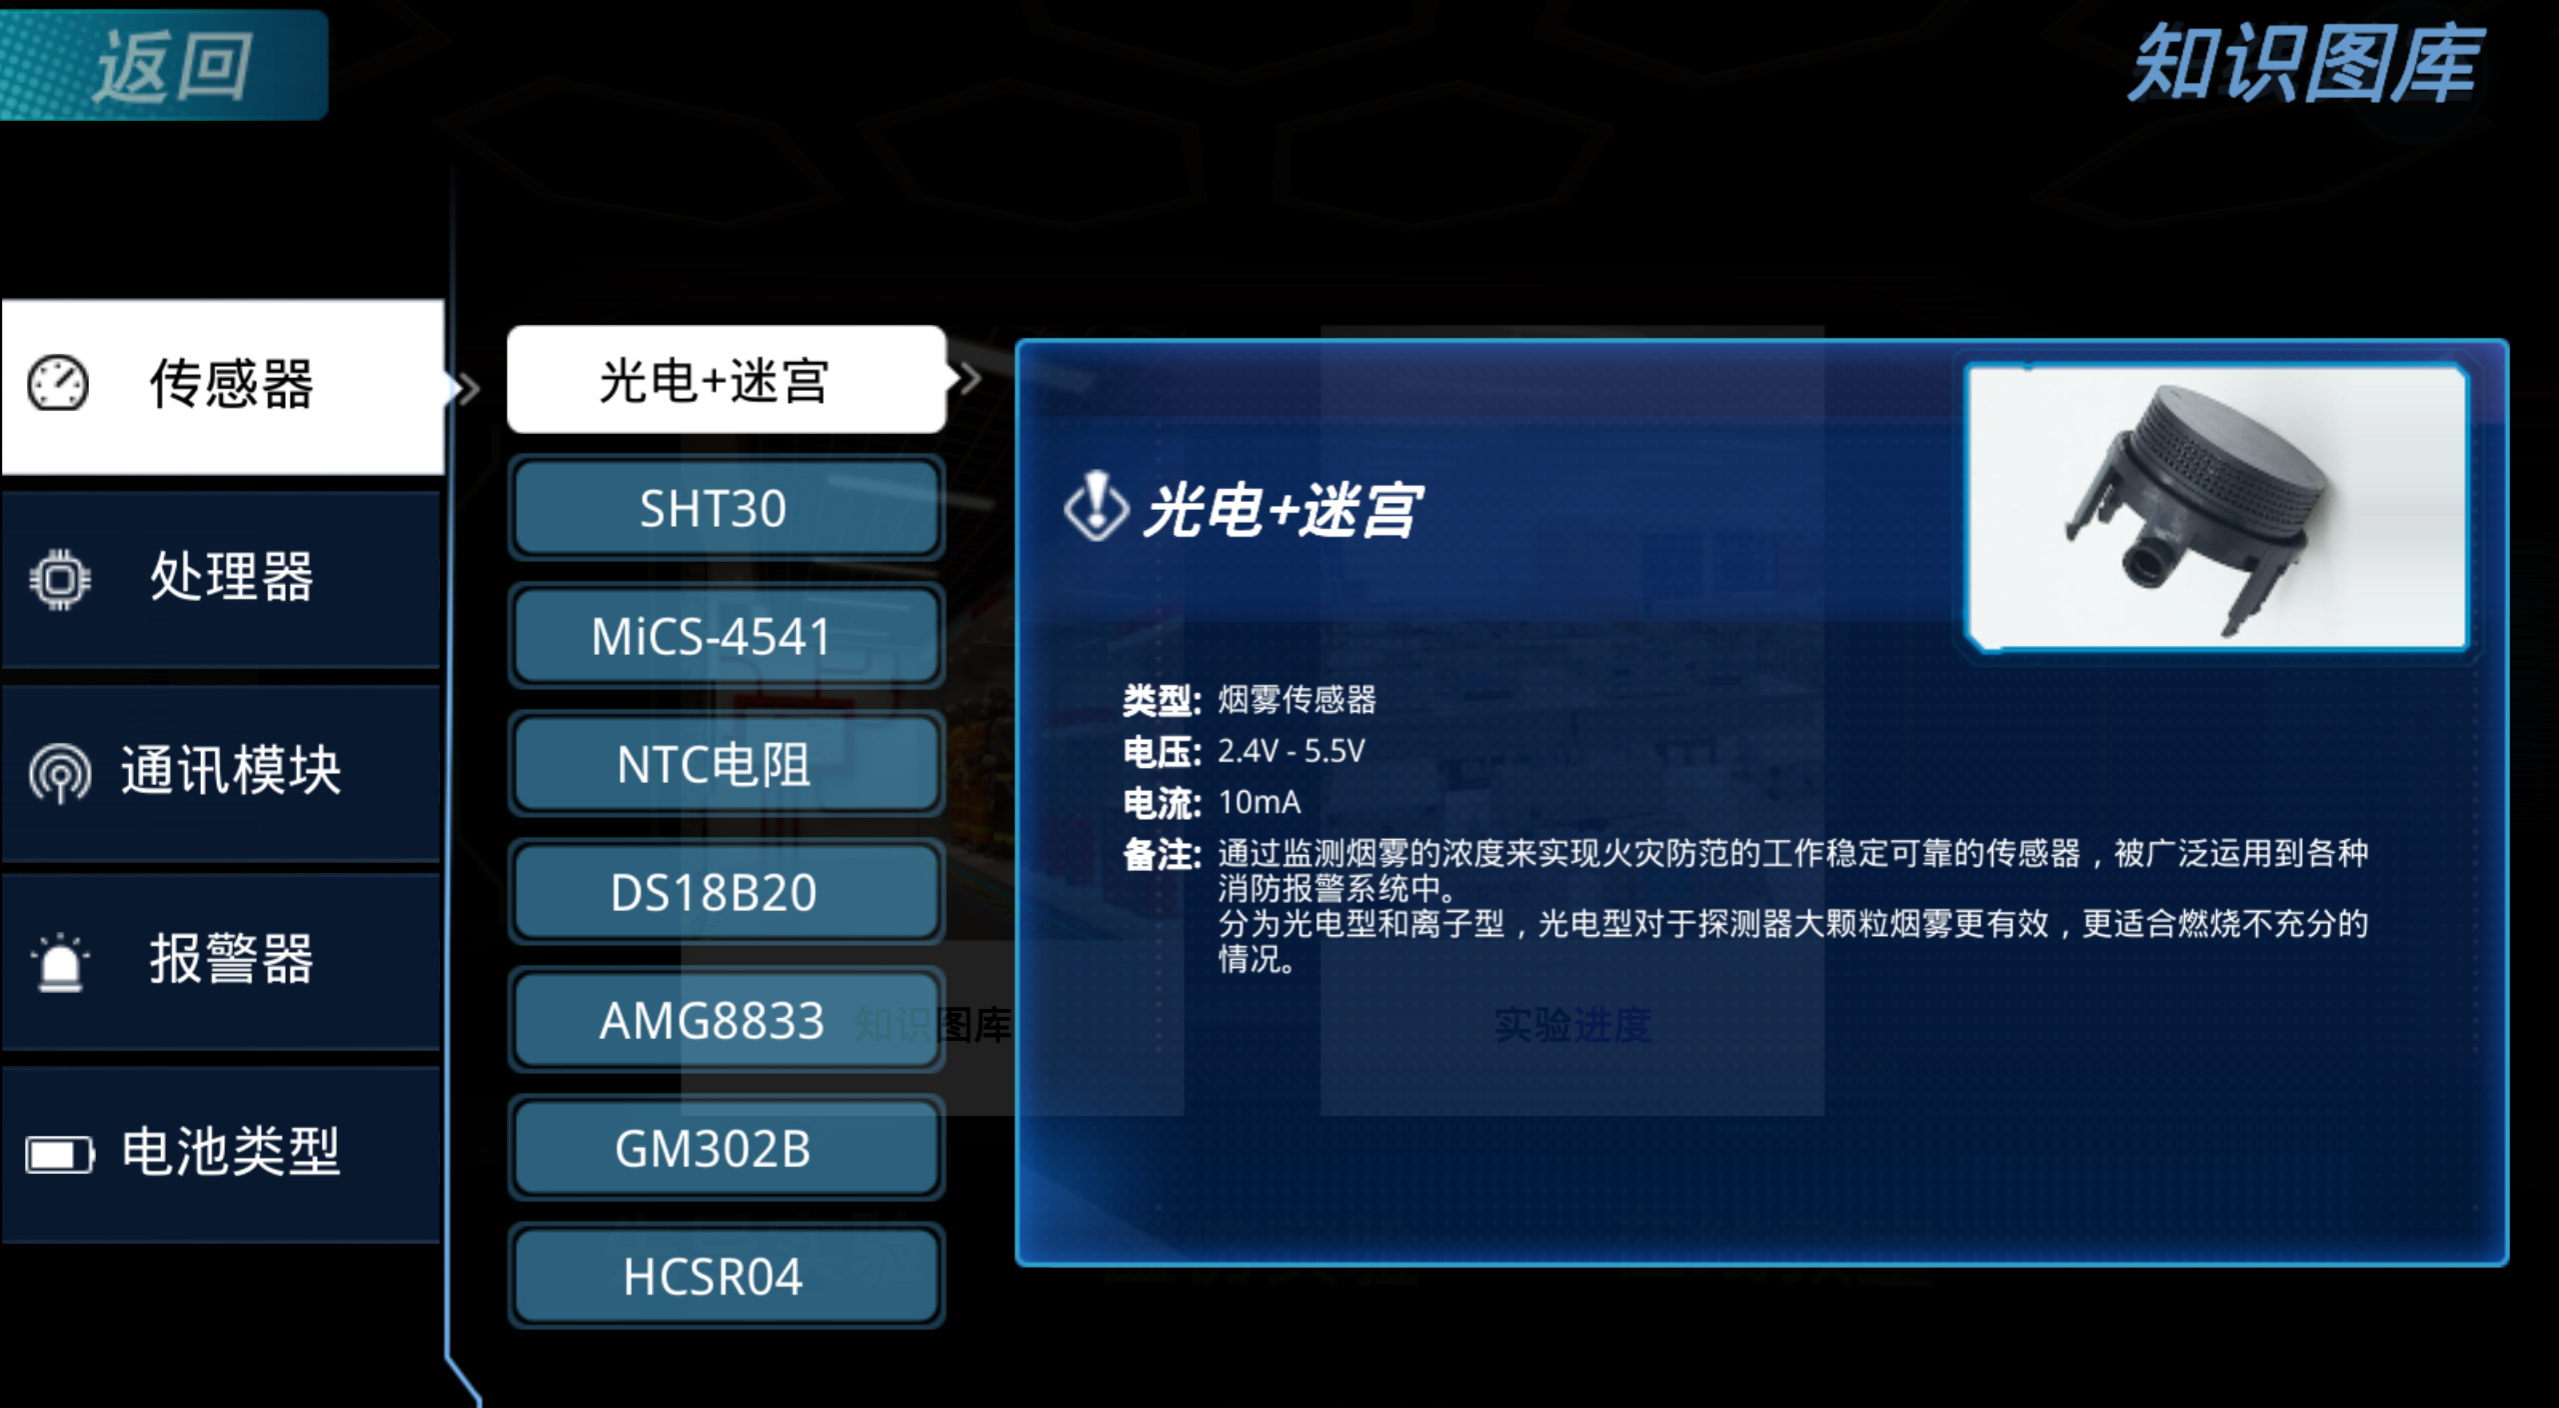
\includegraphics[height=4cm]{fig3}}
    \hfill
    \subfigure[处理器：STM32F103 (Arm Cortex-M3)]{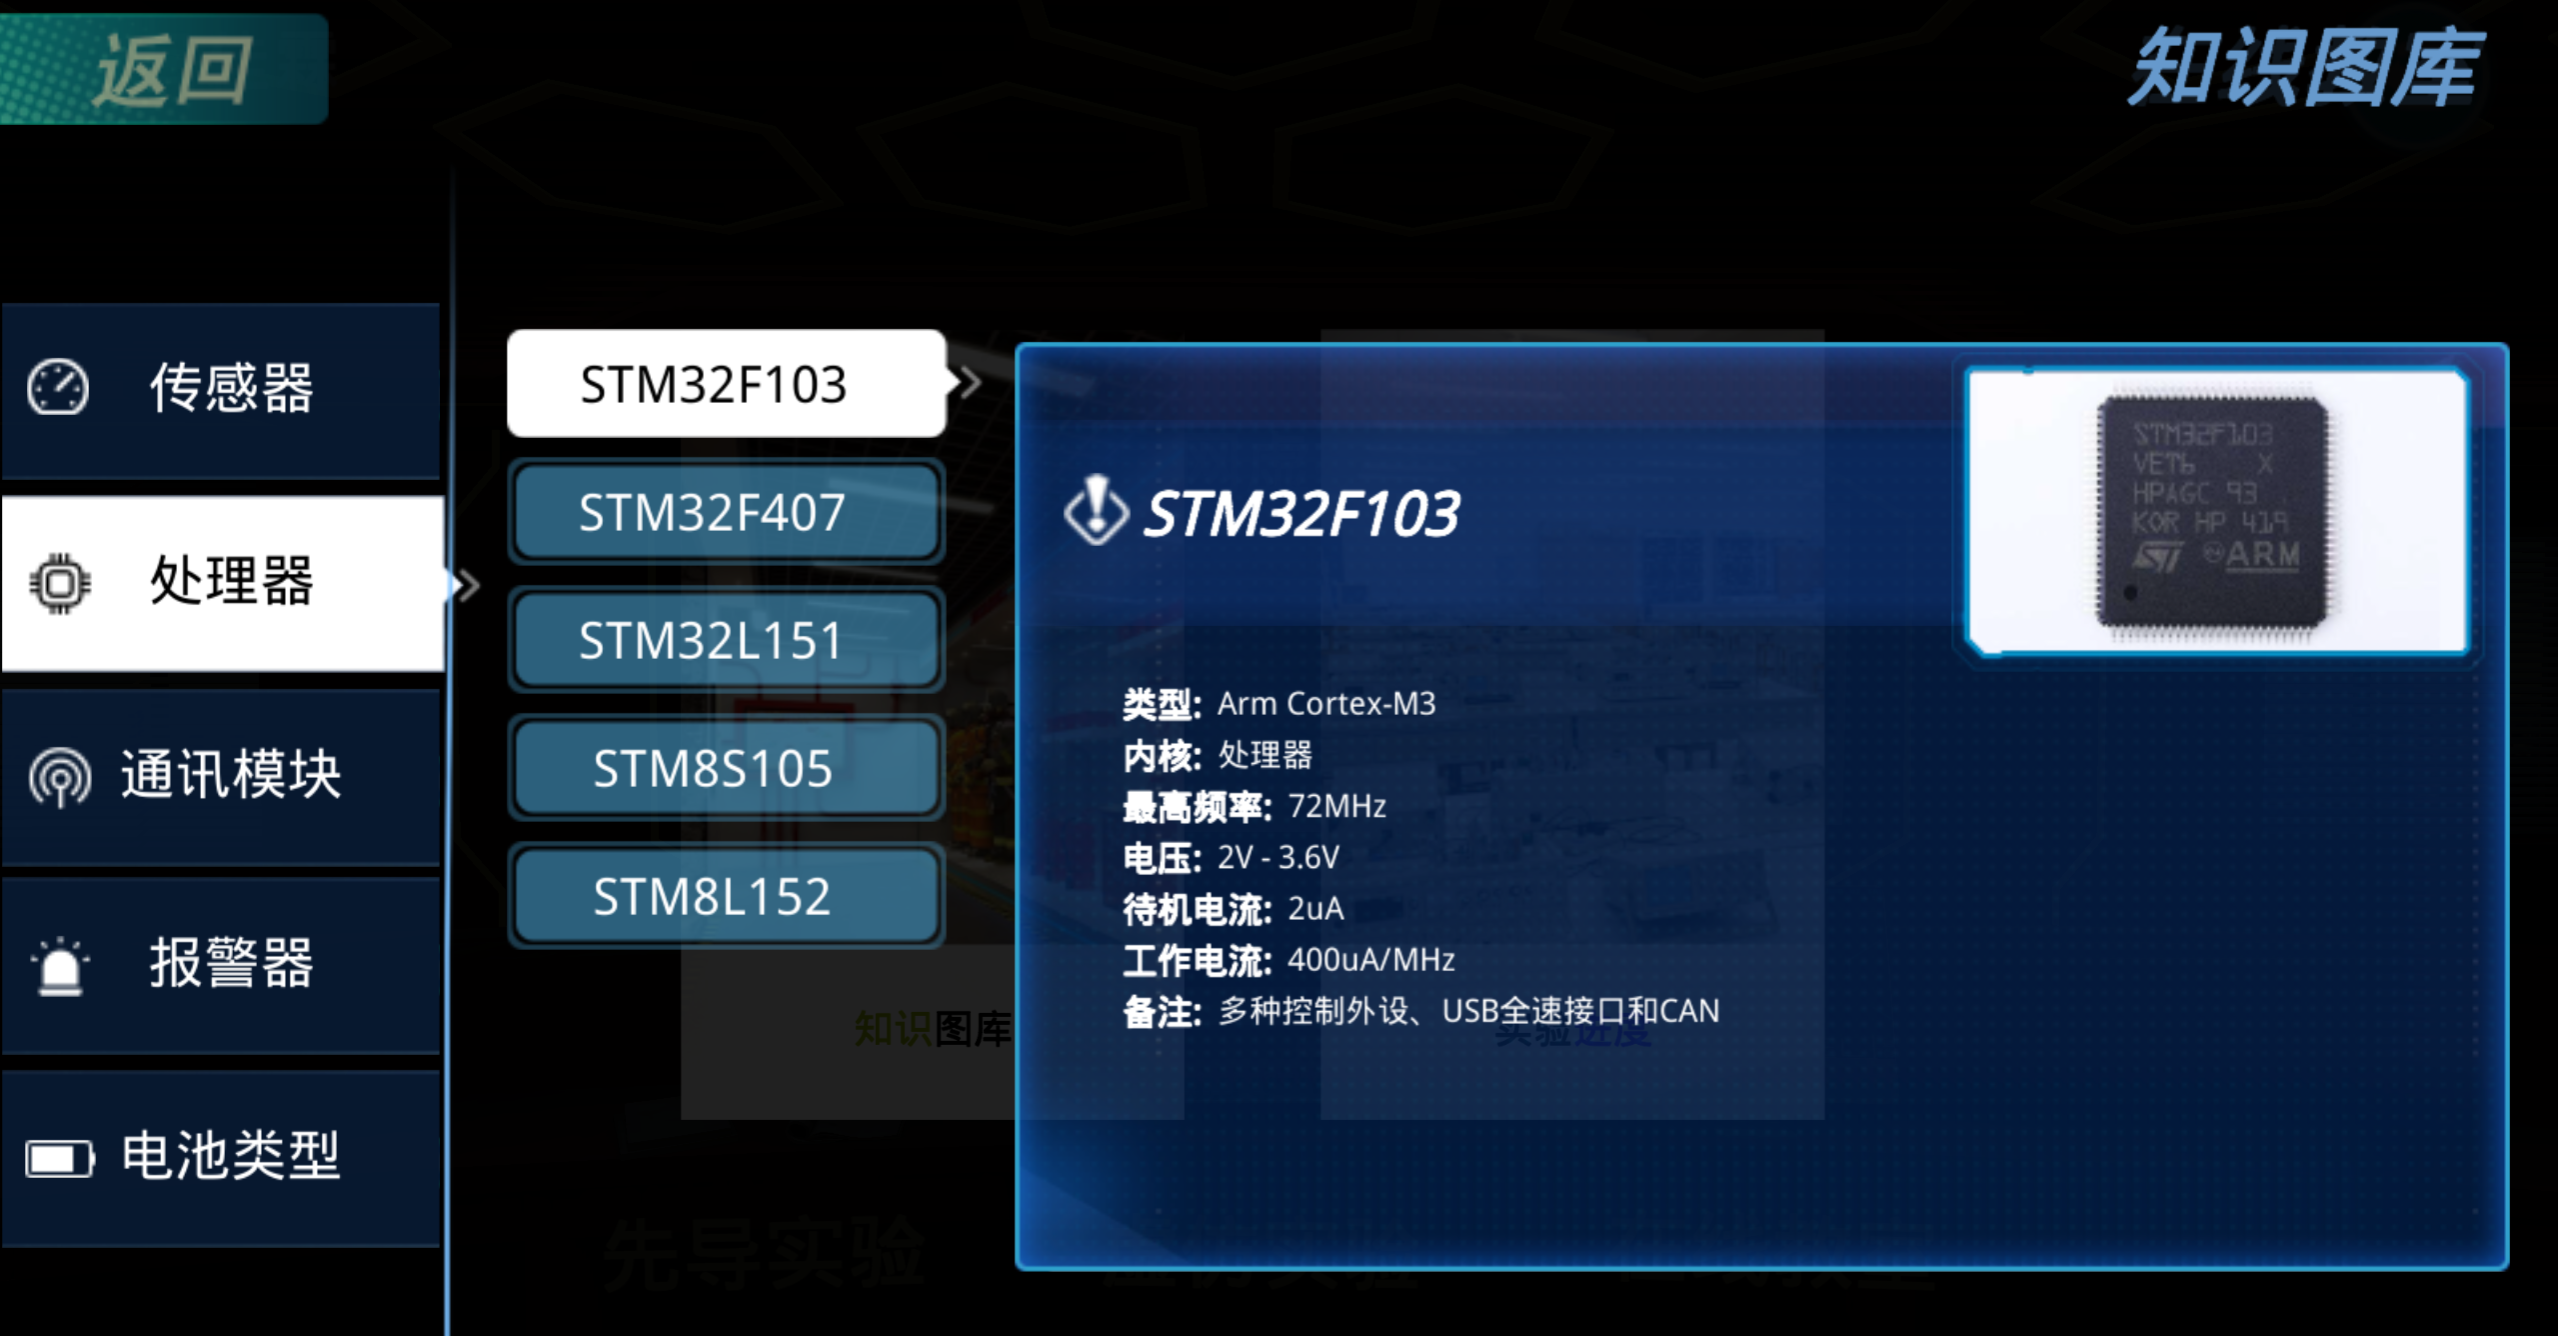
\includegraphics[height=4cm]{fig4}}
    \hfill
    \subfigure[通信模块：NRF24L01 (2.4GHz)]{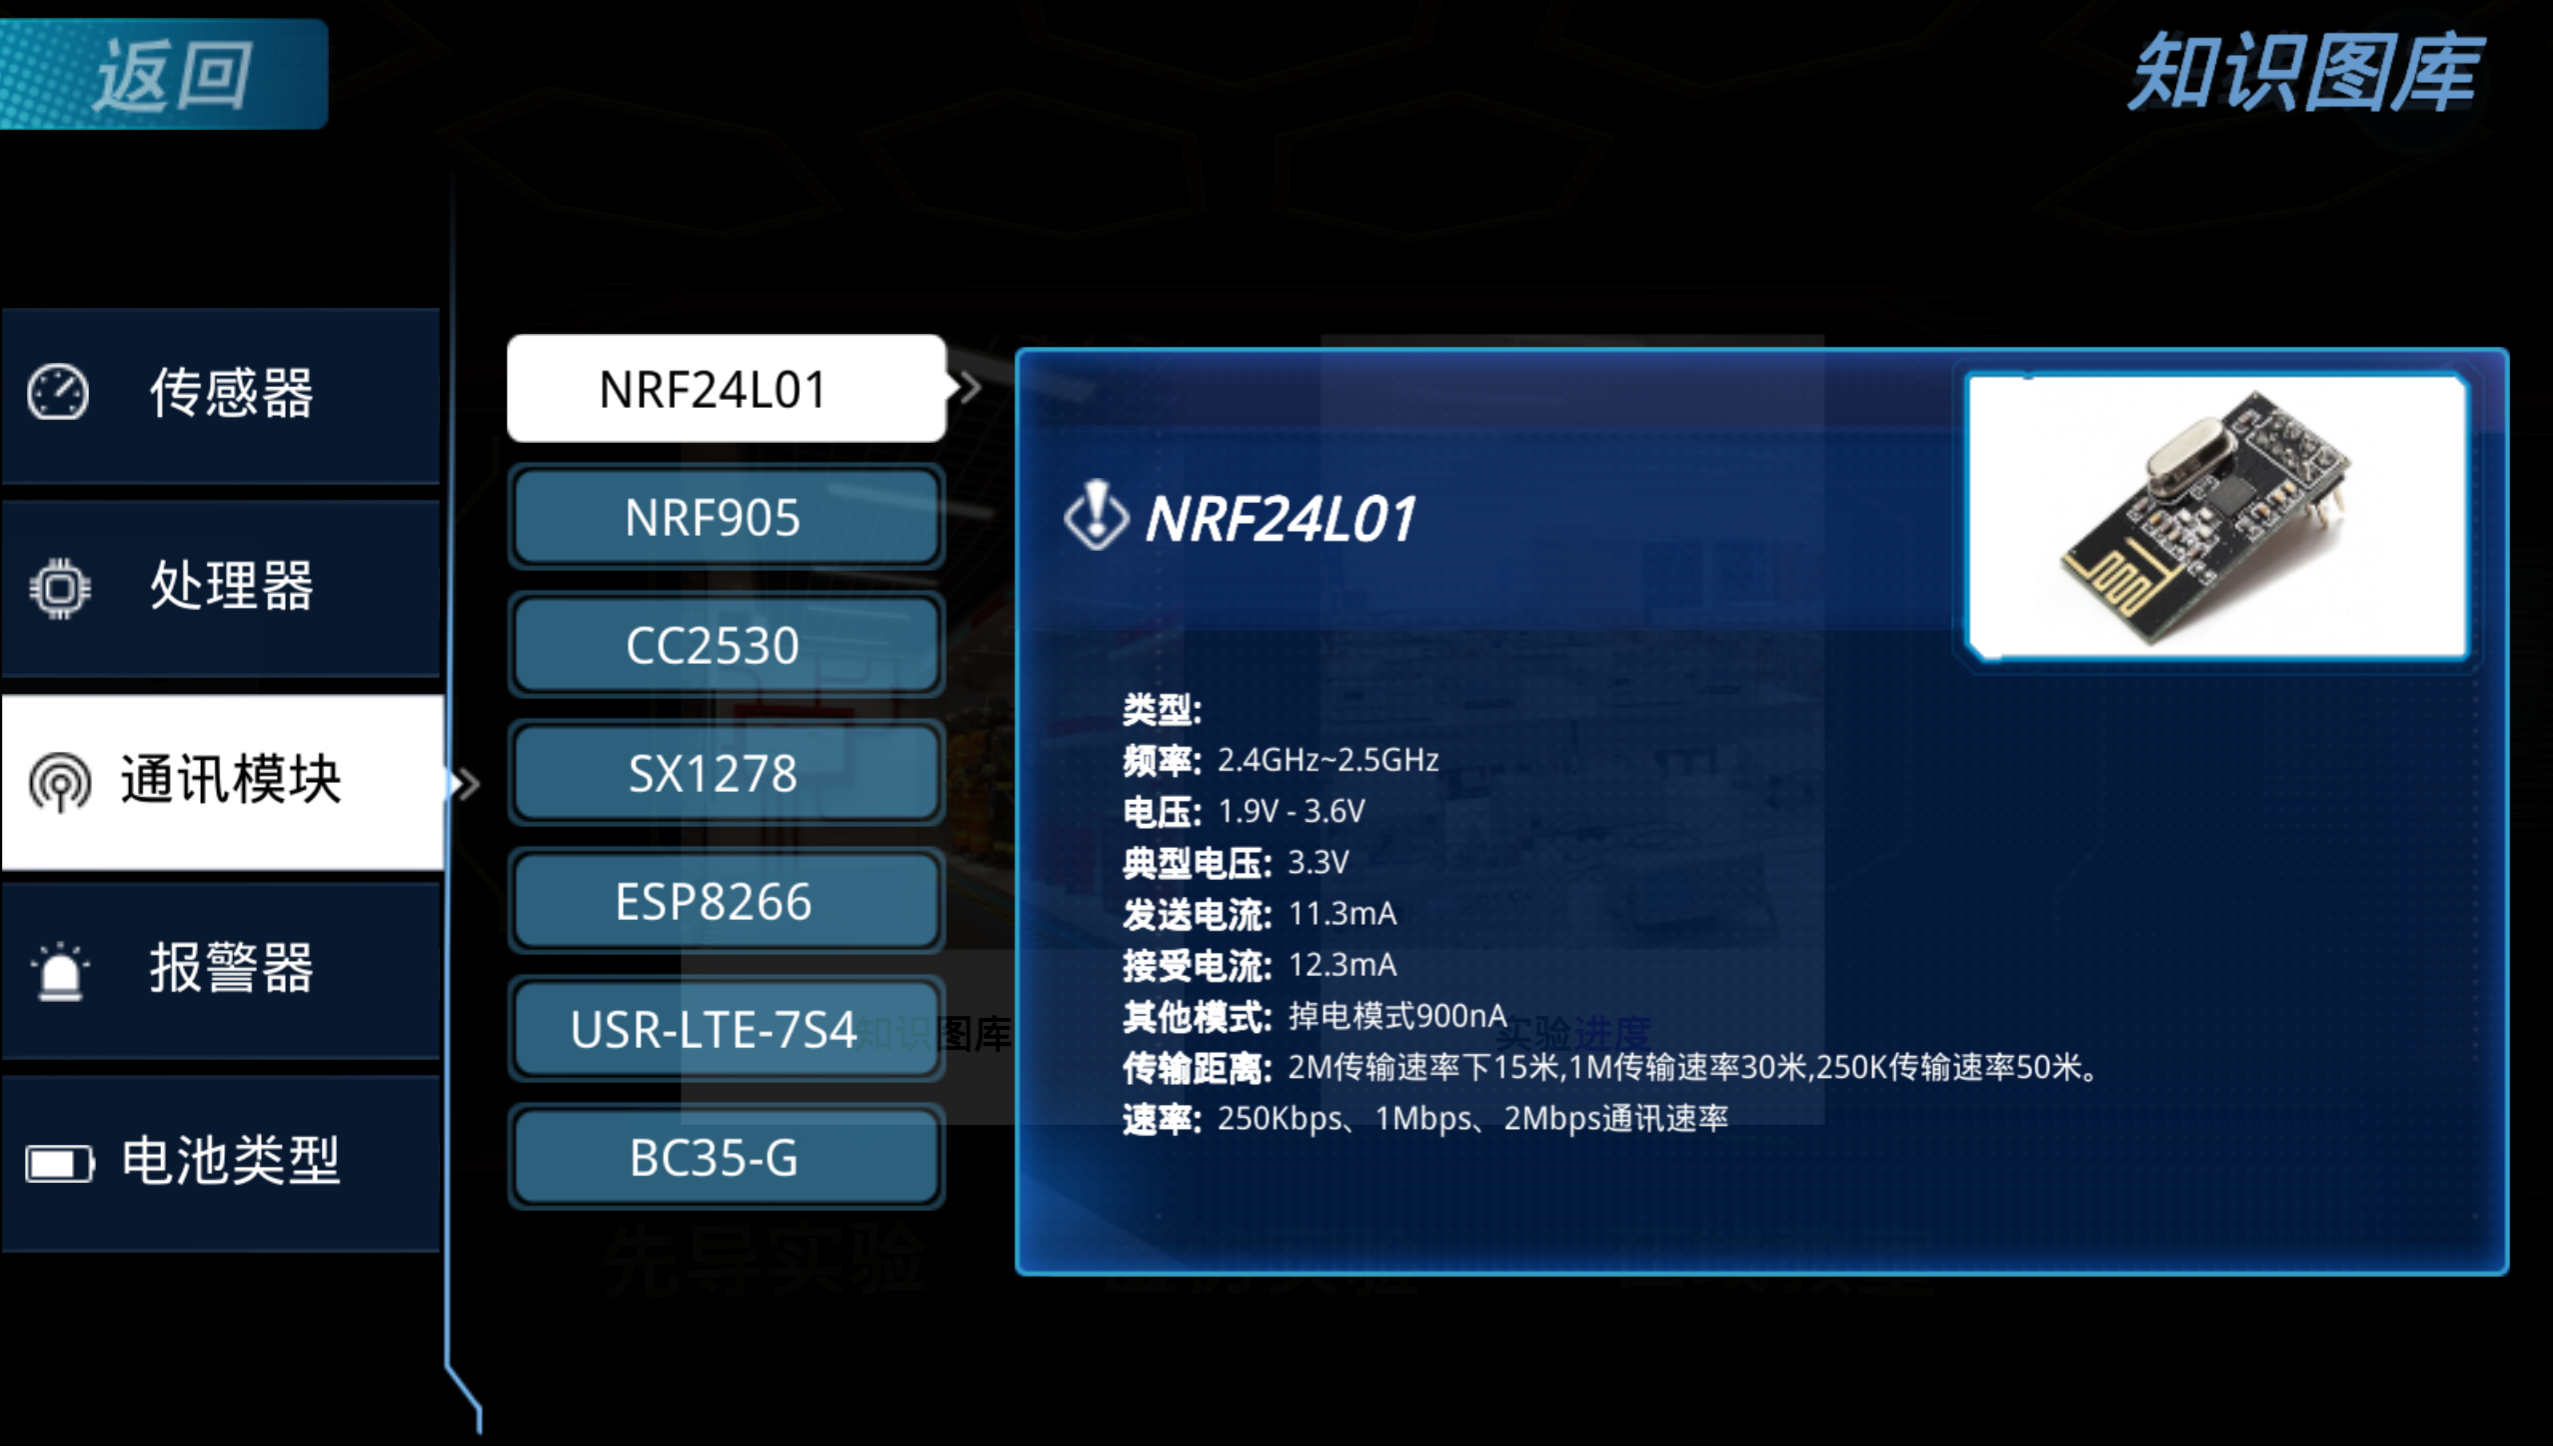
\includegraphics[height=4cm]{fig5}}
    \caption{感知层核心硬件选型知识图谱}
\end{figure}

\begin{table}[H]
    \centering
    \caption{核心器件选型理由与参数说明}
    \renewcommand{\arraystretch}{1.3}
    \begin{tabular}{>{\bfseries}p{3cm} p{4cm} p{7.5cm}}
        \toprule
        \rowcolor{mainblue!10}
        模块分类 & 型号选择 & 选择理由与参数特性 \\
        \midrule
        传感器 (Sensor) & 光电+迷宫探测器 & 电压2.4V-5.5V，工作电流10mA。光电型对大颗粒烟雾更有效，非常适合燃烧不充分的初期火灾探测。 \\
        \midrule
        微控制器 (MCU) & STM32F103 & 最高频率72MHz，待机电流仅2uA。其低功耗特性满足物联网节点电池长期供电的需求，丰富的ADC和外设接口便于采集传感器数据。 \\
        \midrule
        通信模组 (Comm) & NRF24L01 & 掉电模式900nA，发送/接收电流仅11-12mA。适合局域近距离的高效传输（若需远距离可平替为LoRa或NB-IoT模组）。 \\
        \bottomrule
    \end{tabular}
\end{table}

\subsection{软件调试思路与数据流转}
在“做实”方面，除了虚拟搭建，其实际软件运行逻辑至关重要。节点的微控制器(STM32)通过ADC读取光电传感器的模拟量，并进行滤波处理。当烟雾浓度超过设定阈值时，通过SPI接口唤醒NRF24L01/LoRa模块，将报警报文发送至网关。

\begin{lstlisting}[language=C, caption={烟雾传感器ADC读取与报警上报逻辑 (伪代码示范)}]
void Sensor_Task(void) {
    uint16_t smoke_val = ADC_Read(SMOKE_CHANNEL); // 读取烟雾浓度
    smoke_val = Kalman_Filter(smoke_val);         // 滤波防误报
    
    if(smoke_val > THRESHOLD_ALARM) {
        // 触发本地蜂鸣器
        Buzzer_On();
        // 打包数据结构体
        Packet_t alert_pkt = {NODE_ID, TYPE_FIRE, smoke_val, sys_time};
        // 唤醒无线模块并发送
        Radio_Wakeup();
        Radio_Send(LORA_CHANNEL, &alert_pkt);
    }
    Enter_Sleep_Mode(); // 完成后进入休眠，降低功耗
}
\end{lstlisting}


% ================= 第二部分 =================
\section{虚拟仿真实验步骤记录}

在完成核心节点的深入探究后，我按照系统引导完成了全栈（感知、传输、应用）的虚拟实验任务。步骤归纳如下：

\begin{tcolorbox}[colback=white,colframe=gray!50,arc=2mm,boxrule=0.5pt]
\textbf{一、 感知层：无线传感节点虚拟设计}
\begin{itemize}
    \setlength{\itemsep}{0pt}
    \item \textbf{LoRa烟雾节点：} 组装传感器、STM32处理器、LoRa模组、报警器及电池。
    \item \textbf{NB-IoT温湿度节点：} 除硬件组装外，配置了输入/输出电压、总电量及休眠占空比。
    \item \textbf{ZigBee有害气体节点：} 完成搭建并结合“课程思政”与“思考题”进行了扩展学习。
\end{itemize}

\vspace{0.2cm}
\textbf{二、 传输层：场景部署与组网协议设计}
\begin{itemize}
    \setlength{\itemsep}{0pt}
    \item \textbf{网络协议设计：} 针对实验室及“三小场景”（小档口、小作坊、小娱乐场所），自主设计网络框架，配置了传输层与应用层的通信协议。
    \item \textbf{节点部署与联调：} 在虚拟场景的特定点位合理部署温度、烟雾、气体节点。启动系统，验证感知层数据能否成功传输至云服务器并触发警告。
\end{itemize}

\vspace{0.2cm}
\textbf{三、 应用层：应急处理与逃生引导}
\begin{itemize}
    \setlength{\itemsep}{0pt}
    \item \textbf{电气火灾应急：} 模拟多种火情（不同火源与蔓延速度），测试火情监测、云端联动、语音播报及短信推送功能，在规定时间内完成抢险任务。
    \item \textbf{虚拟引导逃生：} 在物联网系统（如应急照明指示牌动态调整）的引导下，规划最优路线并成功逃离火灾现场。
\end{itemize}
\end{tcolorbox}


% ================= 第三部分 =================
\section{实验结果与截图证明}

通过不断的参数调整与逻辑优化，我最终完成了所有的实验任务模块，并生成了实验报告。系统的赋分情况与完成勋章如下：

\begin{figure}[H]
    \centering
    \begin{minipage}[b]{0.48\textwidth}
        \centering
        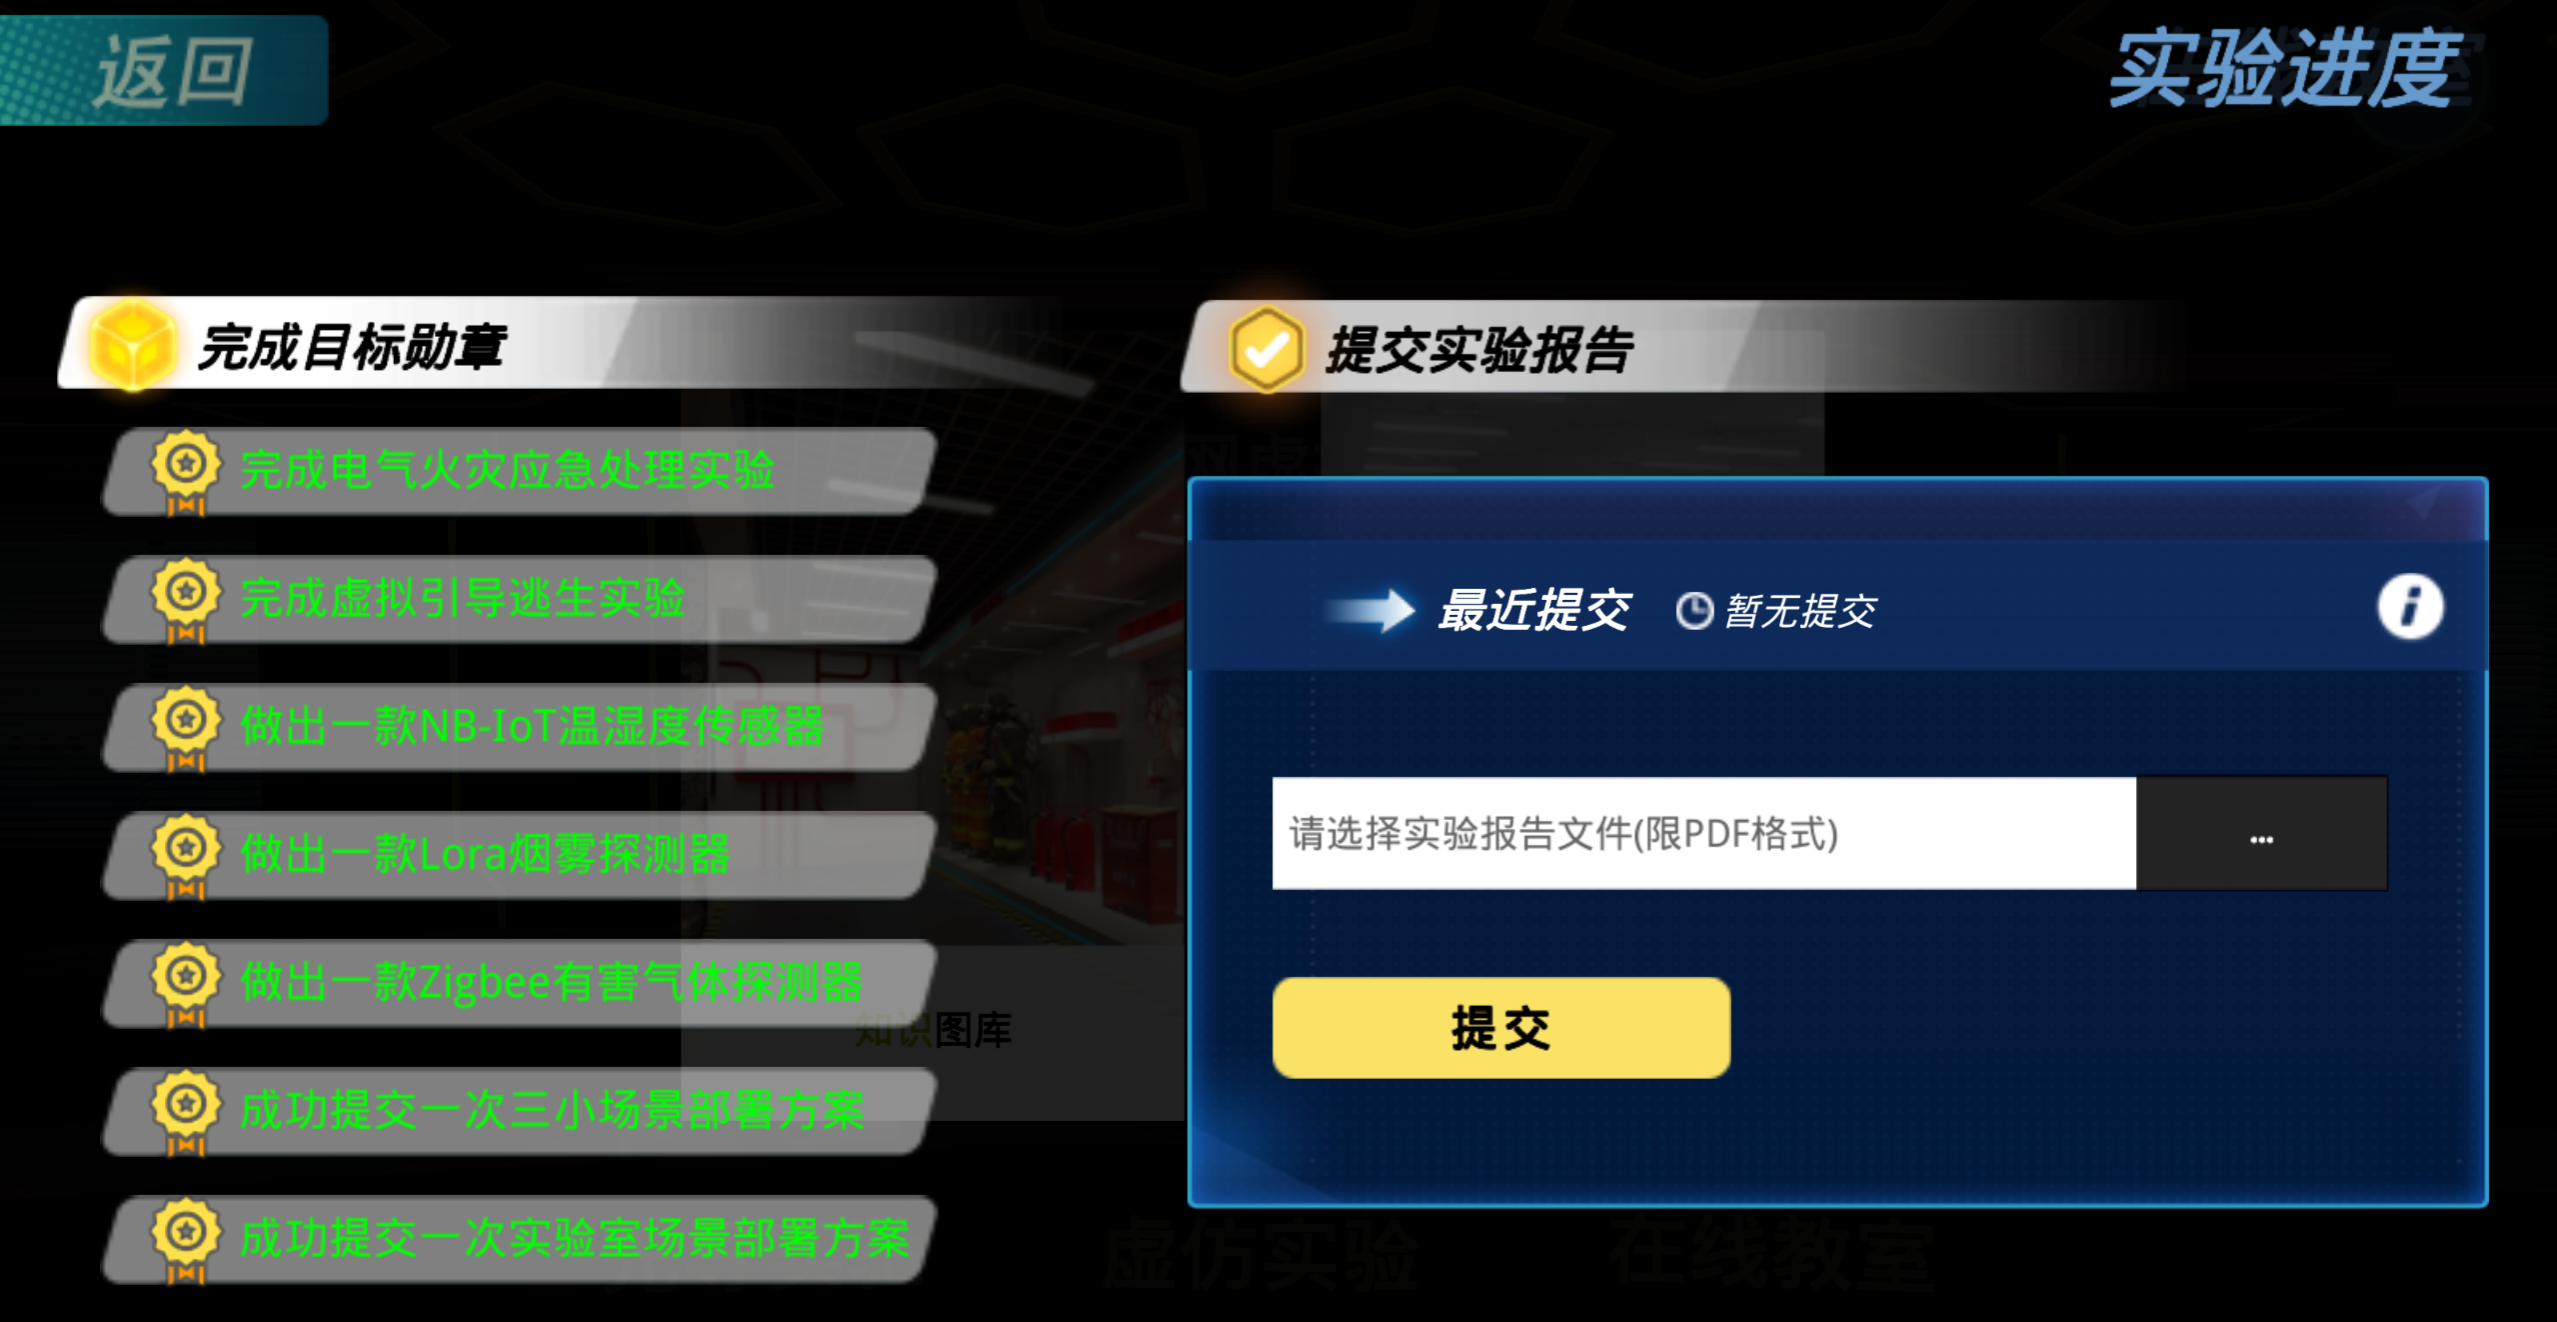
\includegraphics[width=\textwidth]{fig2}
        \caption{当前总成绩面板 (83/100分)}
    \end{minipage}
    \hfill
    \begin{minipage}[b]{0.48\textwidth}
        \centering
        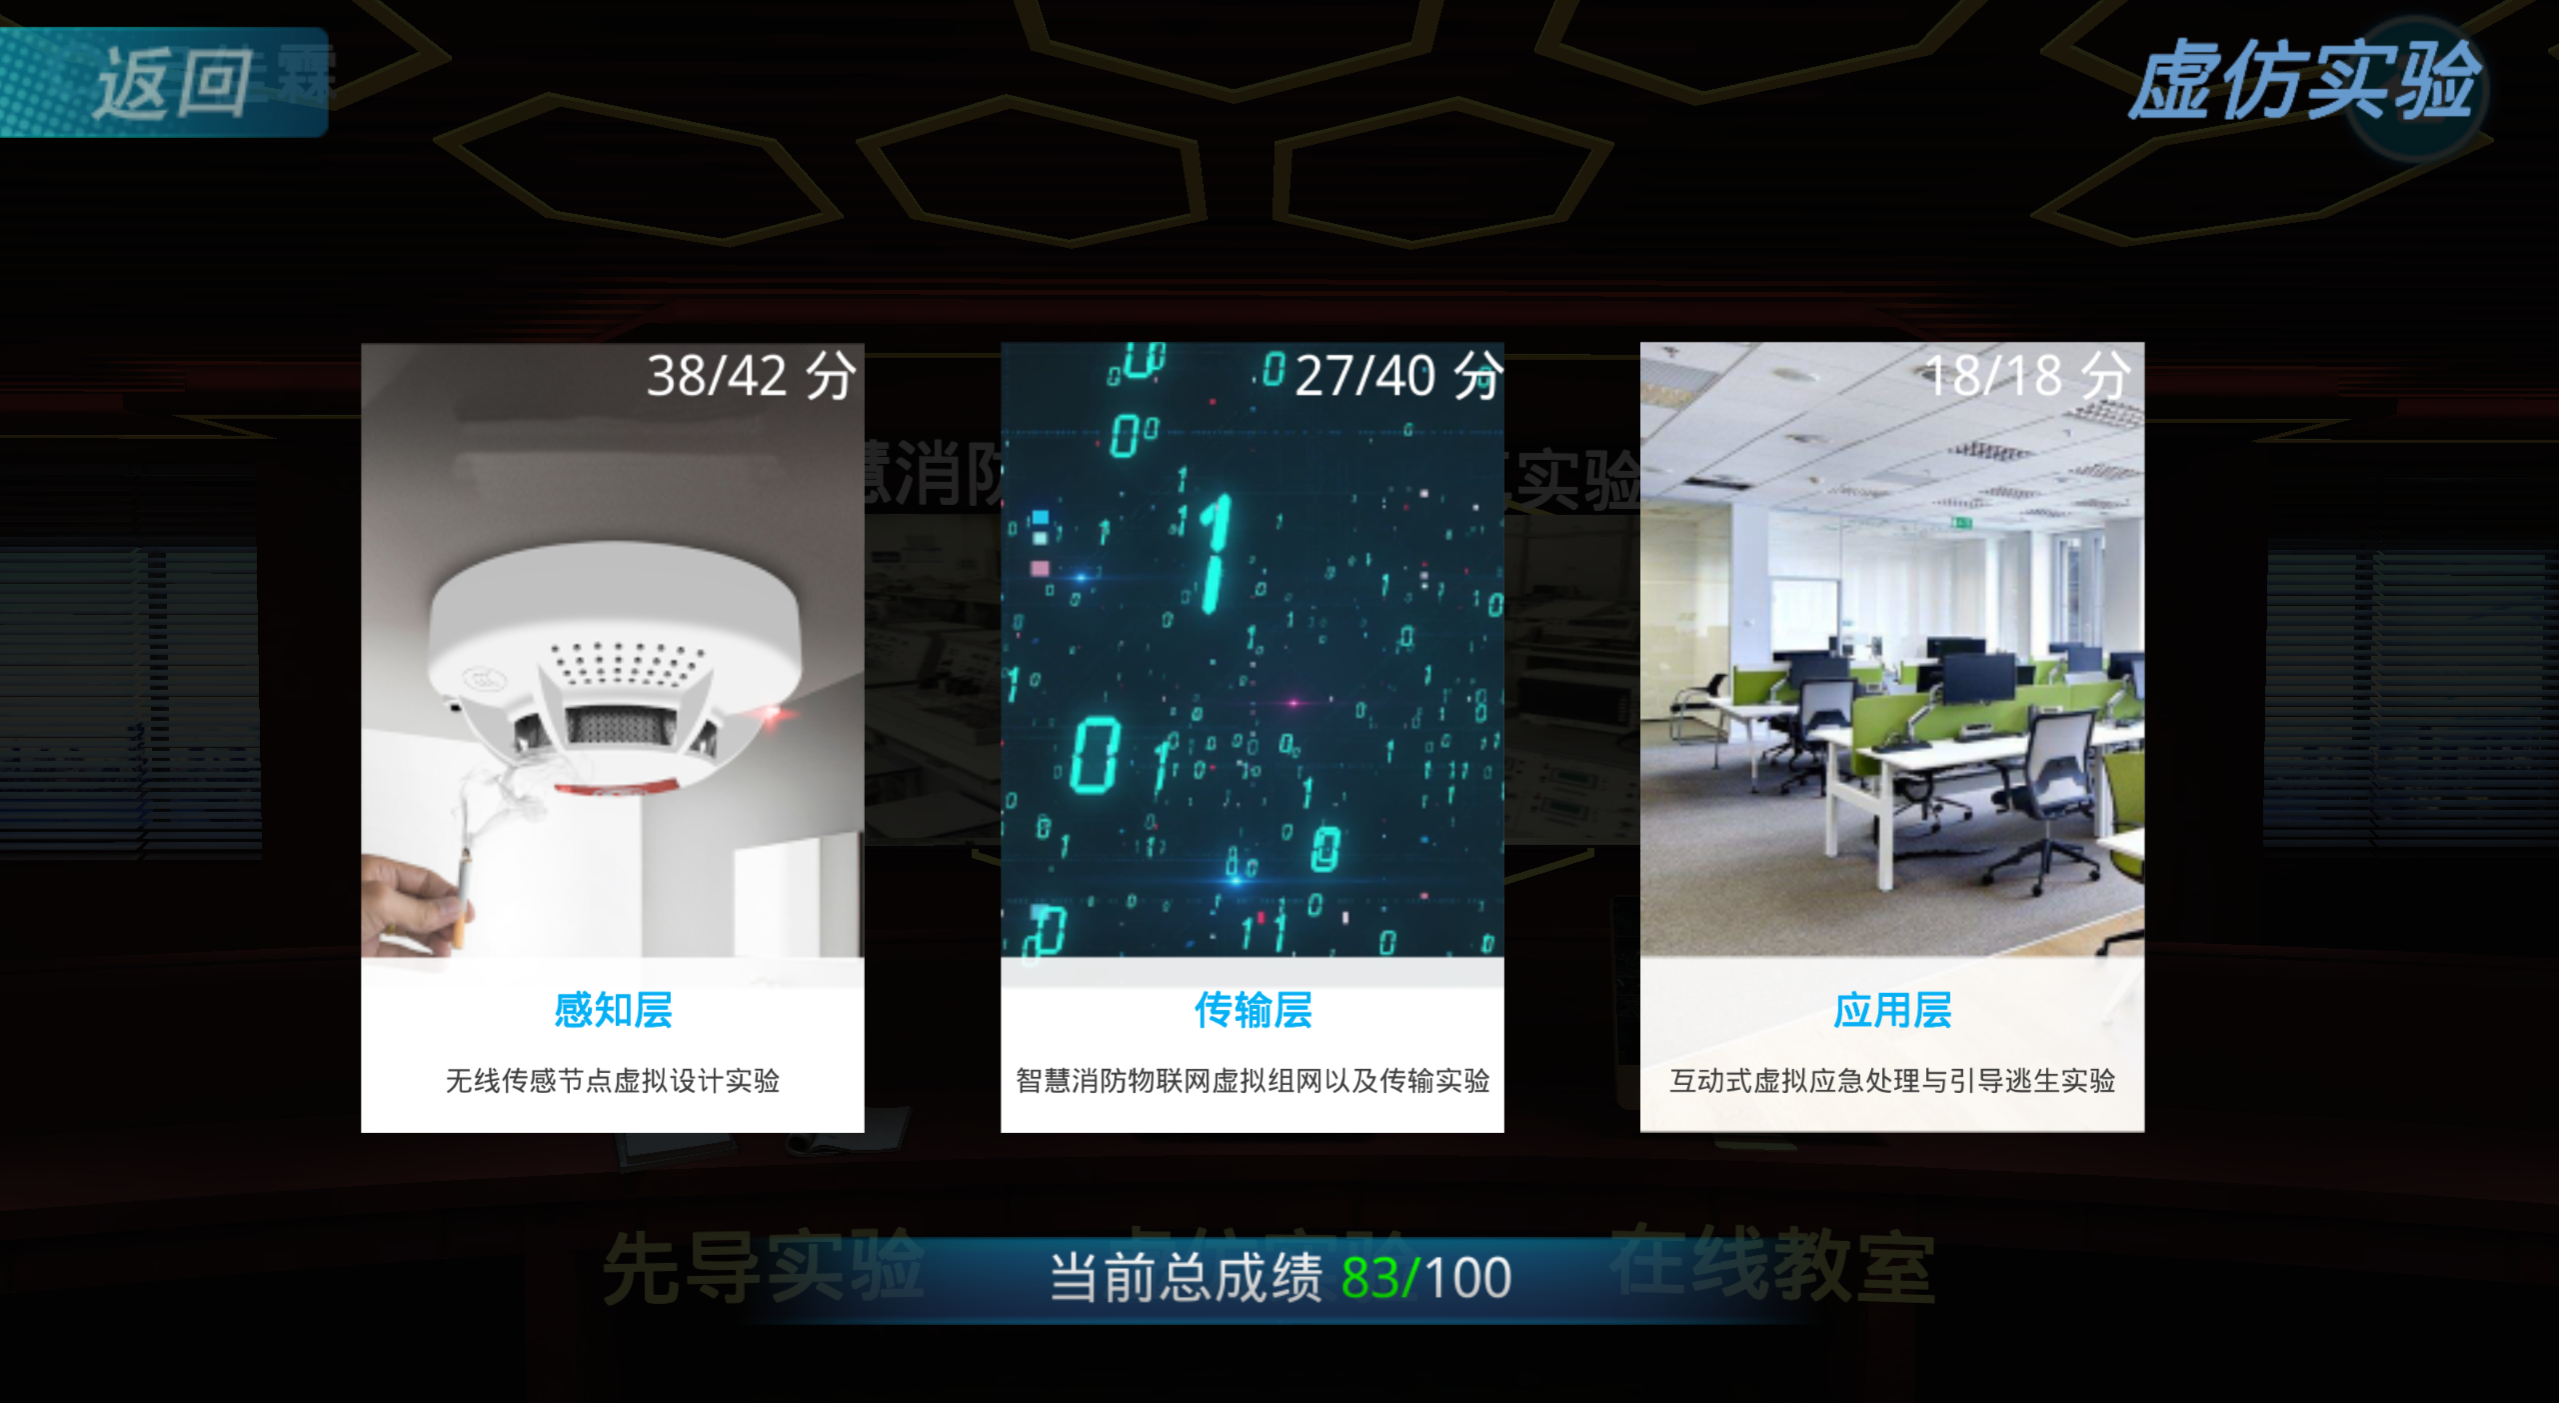
\includegraphics[width=\textwidth]{fig1}
        \caption{完成目标勋章及报告提交页面}
    \end{minipage}
\end{figure}

\textbf{成绩分析：} 
由图2可知，感知层得分38/42，传输层得分27/40，应用层得分满分18/18，总计83分。在传输层网络协议配置及部分硬件组装时（如占空比参数配置）出现过容错扣分，但经过重新设计和累计赋分，最终实现了场景闭环，应用层应急逃生表现完美。图1展示了所有节点开发、场景部署以及逃生实验的“完成目标勋章”。


% ================= 第四部分 =================
\section{心得体会与收获感想}

\begin{tcolorbox}[colback=accentorange!10!white,colframe=accentorange,title=\textbf{实验总结思考},fonttitle=\bfseries]
本次《智慧消防物联网》虚拟仿真实验，让我从枯燥的书本理论跃入了生动立体的工程实践。我有以下三点深刻体会：

\begin{enumerate}
    \item \textbf{专业知识} 正如报告第一部分所剖析的，物联网绝不只是宏观的云平台，它的地基在于每一个光电传感器抗干扰的滤波算法、在于 MCU 低功耗的休眠机制。微小节点的稳定，是整个消防网络不漏报、不误报的核心前提。
    \item \textbf{通信协议的场景适配性} 实验中要求使用 LoRa、NB-IoT、ZigBee 搭建不同节点。我深刻认识到，对于“三小场景”，ZigBee的自组网能力很强；对于深层建筑的烟感，NB-IoT的广覆盖深穿透具有不可替代的优势。技术没有好坏，只有“场景契合度”。
    \item \textbf{科技向善，生命至上} 最后的应用层应急与逃生演练给我触动最深。看着云服务器联动下发的语音播报和动态逃生指示，我真切地感受到物联网代码不仅仅是冷冰冰的 0 和 1，它们在火场中是在与死神赛跑，是守护人民生命财产安全的坚实盾牌。
\end{enumerate}
\end{tcolorbox}

\end{document}